\section{A Digression on Sound}
\subsection{Sound Waves}
Generally, in this class most waves are transverse - ie. the motion is perpendicular to the medium in which the motion is taking place. Sound waves are a notable exception - these are longitudinal waves with motion parallel to the medium. This means the places of highest intensity are compressions in the medium and places of lowest intensity are rarefactions.
\begin{center}
	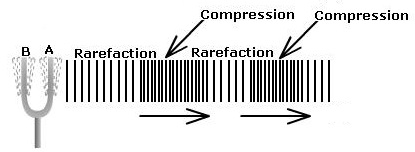
\includegraphics[scale=1.5]{images/waves/soundwaves.jpg}\\
\end{center}
Sound waves exist in three-dimensional space, and so the wavefront of a sound wave is the surface of a sphere, of which the total energy in the sound wave must be distributed over. The surface area of the wavefront is proportional to the square of the distance $r$ from the source, so the intensity of the wave goes down as $\frac{1}{r^2}$. In order to achieve this, we model the wave as a spherical Bessel wave of the form $y(r, t) = \frac{\sin(kr-\omega t)}{r}$, where $r$ is the distance from the source. This is derived from the fact that intensity is proportional to energy times amplitude $A$ squared, and hence $A \propto \frac{1}{r}$. The "amplitude" can also be thought of how far points in the medium are displaced from equilibrium.
\section{Interference and a "Double Slit Experiment"}
It's instructive to see how sound waves interfere with each other, especially since these are spherical waves. This is exemplified in the sound version of the "double-slit experiment", where we place two speakers a distance $d$ apart and measure intensity of the sound on a line a distance $D$ away. 
\begin{center}
	\begin{asy}
		import graph;
		size(175); 
real wall = 5; 
real D = 9;
real y = 4;
real d = 1.5;
pair sp1 = (0, d); 
pair sp2 = (0, -d); 
draw(Circle(sp1, 0.1)); 
draw(Circle(sp2, 0.1)); 
draw((D, -wall)--(D, wall)); 
draw((0, wall)--sp1+dir(90)*0.2, linetype("4 4")); 
draw((0, -wall)--sp2+dir(270)*0.2, linetype("4 4")); 
draw(sp2+dir(90)*0.2--sp1+dir(270)*0.2, linetype("4 4")); 
dot((D, y)); 
dot((0, 0)); 
draw((0,0)--(D, 0), linetype("4 4")); 
draw((0, -4)--(D, -4), Arrows);
dot((D, 0));
draw((D+0.5, 0)--(D+0.5, y), Arrows); 
draw((-0.5, d)--(-0.5, -d), Arrows);
draw(sp1+dir(25)*0.2--(D, y));
draw(sp2+dir(40)*0.2--(D, y));
draw((0, 0)--(D,y), linetype("8 8")); 
for (int r = 0; r < 3; ++r)
{
	draw(arc(sp1, 0.4+0.2*r, 60, -60));
	draw(arc(sp2, 0.4+0.2*r, 60, -60));
}
label("$d$", (-0.5, d)--(-0.5, -d), W);
label("$R$", (0,0)--(D,y), dir(140));
label("$y$", (D+0.5, 0)--(D+0.5, y), E);
label("$D$", (0+0.2, -4)--(D-0.2, -4), S);
label("$\theta$", (0,0), dir(12)*7);
	\end{asy}
\end{center}
For some arbitrary point $y$ from the center on the line, let $R$ be the distance from the midpoint of the sound sources to this point, and $\theta$ to be the angle between the line to this point and the perpendicular to the line. \\
Using our model for sound waves (Bessel waves) discussed in the previous section, from our arbitrary point, we can compute the wave experienced at this point as the sum of two sound waves (in exponential form): 
\[
	u(y, t) = \frac{1}{2} \left[ \frac{e^{i \left(k \sqrt{D^2 + \left(y - \frac{d}{2} \right)^2} - \omega t\right)}}{\sqrt{D^2 + \left(y - \frac{d}{2} \right)^2}} + \frac{e^{i \left(k \sqrt{D^2 + \left(y + \frac{d}{2} \right)^2} - \omega t\right)}}{\sqrt{D^2 + \left(y + \frac{d}{2} \right)^2}} \right] 
\]
Note that taking the imaginary part of this expression will result in the sum of the waves we desire. Since we're mostly concerned where the maximum/minimum intensities are, we can use this exponential form of the wave to describe the wave. We also include the factor of $\frac{1}{2}$ to normalize the wave - it will scale the actual magnitude of the wave down by a factor of $2$, but it will not have an effect on which points will have a maximum/minimum intensity.\\
We will now make the approximation that $D >> d$, and use the Taylor series of the square root term, using the two lowest-order terms: 
\begin{align*}
	\sqrt{D^2 + \left(y - \frac{d}{2} \right)^2} &= \sqrt{D^2 + y^2 - yd + \left( \frac{d^2}{4} \right)} \\
	&= R \sqrt{1 - \frac{yd}{R^2} + \frac{d^2}{4R^2}} \\
	&= R \left[1 + \frac{1}{2}\left(\frac{d^2}{4R^2} - \frac{yd}{R^2}\right) - \frac{1}{8}\left(\frac{d^2}{4R^2} - \frac{yd}{R^2}\right)^2 + \ldots \right] \\
	&\approx R\left[1 - \frac{yd}{2R^2} \right] 
\end{align*}
We plug this approximation back into our original expression, using a similar approximation for the other square root. We also use $R$ to approximate the radicals in the denominator: 
\begin{align*}
	u(y, t) &= \frac{1}{2R} \left[ e^{i \left(kR - \frac{kyd}{2R} - \omega t\right)} + e^{i \left(k R + \frac{kyd}{2R} - \omega t\right)} \right] \\
	&= \frac{e^{i \left(kR - \omega t\right)}}{2R} \left[ e^{- i\frac{kyd}{2R}} + e^{i\frac{kyd}{2R}} \right] \\
	&= \frac{e^{i \left(kR - \omega t\right)}}{R} \cos \left( \frac{kdy}{2R}\right) = \frac{e^{i \left(kR - \omega t\right)}}{R} \cos \left( \frac{kd}{2} \sin \theta \right)
\end{align*}
From this, we can see that we can maximize/minimize the amplitude, and thus, the intensity of the sound if we maximize/minimize the cosine term. \\
When the intensity of the sound is observed to be at a maximum, we should have that the argument of the cosine function should be $n \pi$ for some integer $n$ to have a maximum magnitude. This implies:
\[
	\frac{kd}{2}\sin \theta = n \pi  \rightarrow \frac{\pi d}{\lambda}\sin \theta = n \pi \rightarrow d\sin \theta = \lambda n 
\] 
Similarly, when the intensity of the sound is observed to be a minimum, the argument of the cosine function should be $\left( n + \frac{1}{2} \right) n$ for some integer $n$, so the magnitude of the intensity is minimized when:
\[
	\frac{kd}{2}\sin \theta = \left( n + \frac{1}{2} \right) \pi  \rightarrow \frac{\pi d}{\lambda}\sin \theta = \left( n + \frac{1}{2} \right) \pi \rightarrow d\sin \theta = \lambda \left( n + \frac{1}{2} \right) 
\]
\subsection{Modulation and Carrier Waves}
When dealing with sound waves in particular, we can see what happens when we look at interference of sound waves with different frequencies instead of looking at spatial differences in the double-slit experiment.\\
Consider two waves with angular frequencies of 12 Hz and 2 Hz. (These are not sound waves you can hear, but it doesn't impede our mathematical calculations.) If we consider the sum of two waves (ignoring spherical nature of sound waves), we see that, by sum-to-product identities:
\[
	\sin(12t) + \sin(2t) = 2\sin(7t)\cos(5t)
\]
If we look at the graph of this function: 
\begin{center}
	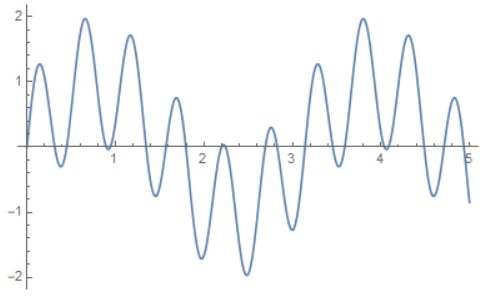
\includegraphics[scale=1]{images/waves/modulation1.jpg}\\
\end{center}
we see that the overall wave has an angular frequency of 2 Hz, but inside the wave itself there are waves oscillating at a frequency of 12 Hz still. If one were to play a scaled up version of these waves to audible frequencies, one could hear both of these distinct sounds (try, for example, a high C and a low A). \\
Let's also consider two waves with closer angular frequencies, say 22 Hz and 20 Hz. By a similar manipulation we can see that: 
\[
	\sin(22t) + \sin(20t) = 2\sin(21t)\cos(t)
\]
See the graph of this function below: 
\begin{center}
	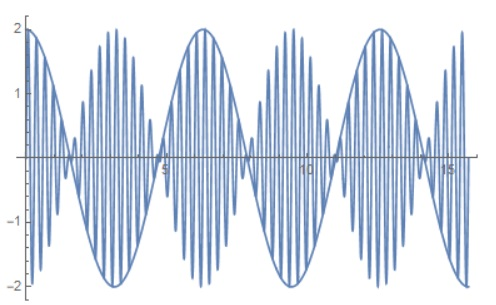
\includegraphics[scale=1]{images/waves/modulation2.jpg}\\
\end{center}
Here, we see that the resultant wave exhibits neither a frequency of 22 Hz nor 20 Hz. Internally, the wave exhibits a frequency of 21 Hz, while overall, the wave moves along with a frequency of 2 Hz. (Notice that this is not simply 1 Hz!) This wave that carries an overall frequency of 2 Hz is called the carrier wave. If we graph $\cos(t)$ directly on top of the function, as shown, this function envelops our combination of two waves perfectly, but it doesn't have the same frequency as the carrier wave - in fact, it has half of the correct frequency. This phenomenon only occurs if the frequencies are sufficiently close enough (and we can hear it in real life if we play a C and a G together, which will sound like an E with a modulating tone beneath that will make it sound like there's a beat within the note). \\
Therefore, when we play two sound waves together, the resultant waves can either mesh together into a single wave and frequency with a modulating frequency determined by a carrier wave, or will noticeably be two separate waves with the same frequencies as before. In each scenario, they will sound different (two tones vs. one tone) based on how close together these frequencies are. 
